\documentclass[./dissertation.tex]{subfiles}
\begin{document}
\newpage\null\thispagestyle{empty}\newpage
    \chapter{Complex and $\mu$-Processor Based Systems}
\section{Introduction}
\label{introduction}
In the last years the density of integration in VLSI systems and microprocessors performances have continuously increased, thanks to the relentless technology scaling. Even though this trend can only continue on its path, several constraints may obstruct the way (power, energy, performance), in particular \textit{reliability} (or cross-layer resilience) can become the more relevant. Hardware redundancy can be used to manage errors at the hardware architecture layer, and eventually even software implemented error detection and correction mechanisms can manage those errors that escalated from the lower layers of the stack \cite{7544311} \cite{6560692}. Overall, the goal is to determine the resilience of a particular system in determined conditions, meeting the requirements considering its sensitivity to hardware faults.

It is also true that software failures are not only caused by software implemented faults, as it has been shown \cite{6258310} the propagation of hardware faults plays a central role, eventually catastrophic. Base on what literature reports on hardware faults evaluation reports \cite{EBRAHIMI20141000} \cite{7604674} it is possible to observe that the percentage of software failure that are caused by pure hardware faults average around 10\% \cite{kooli:lirmm-01693156}. The most famous example is surely the crash of the Mars Polar Lander \cite{1181509}, which cause was established to be dependant on hardware faults resulting in software failure. In that case the lander was not able to settle the legs into their deployed position, which is an hardware fault, and the software gave a wrong order to turn off the engines in the air of Mars, which is a software fault. The system crashed and the entire mission failed.

This paper not only wants to furthermore analyse the behaviour of software failure due to hardware propagated fault but parallely  to the main research \cite{9486705} path that applies these new methodology to Hardware design in order to simplify the reliability assessment, the idea of applying the same method in the scope of the assessment of the reliability of software has never been tested. In order to do so, there is the need to specify the main characteristic that Software Products have, fundamental to lay the basis for the described work. Every software can be divided into basic block, atomic chunks of software having the following proprieties:
\begin{itemize}
    \item One entry point, meaning no code within it is the destination of a jump instruction anywhere in the program.
    \item One exit point, meaning only the last instruction can cause the program to begin executing code in a different
basic block.
\end{itemize}
Under these circumstances, whenever the first instruction in a basic block is executed, the rest of the instructions are
necessarily executed exactly once, in order.
The code may be source code, assembly code, or some other sequence of instructions.
More formally, a sequence of instructions forms a basic block if:
\begin{itemize}
    \item The instruction in each position dominates, or always executes before, all those in later positions.
    \item No other instruction executes between two instructions in the sequence.
This definition is more general than the intuitive one in some ways. For example, it allows unconditional jumps to
labels not targeted by other jumps. This definition embodies the properties that make basic blocks easy to work with
when constructing an algorithm.
\end{itemize}

The blocks to which control may transfer after reaching the end of a block are called that block’s successors, while the blocks from which control may have come when entering a block are called that block’s predecessors. The start of a basic block may be jumped to from more than one location.
Laid these basis, if, as we'll show in this paper, the reliability metrics extracted for each basic block can be recomposed just knowing the sequence of block required to execute a precise operation, the need for a fault injection campaign on the entire software product doesn't stand anymore.

This paper is organised as follows: the current state of the art is summarised in section II; section III describes the proposed methodology, including its setup, the fault injection procedure and the re-composition of the results from each basic block; a test case is provided in Section IV, while Section V presents the obtained results and sketches some perspectives.
%
%~~~~~~~~~~~~~~~~~~~~~~~~~~~~~~~~~~~~~~~~~~~~~~~~~~~~~~~~~~~~~~~~~~~~~~~~~~~~
%                       STATE OF THE ART 
%~~~~~~~~~~~~~~~~~~~~~~~~~~~~~~~~~~~~~~~~~~~~~~~~~~~~~~~~~~~~~~~~~~~~~~~~~~~~
%
\section{State of the Art}
The rush to develop a methodology to assess the reliability and availability of electronic systems has speed up together with the increasing complexity of the microelectronic systems and the miniaturization of such devices. In particular an eye has been keep onto the propagation of faults throughout the entire stack of layers that compose the system as whole, starting from the technological layer all the way up to the software/application layer passing through hardware. 
In particular the extraction of reliability metrics for software has been the focus of a consistent thread of research \cite{kooli:lirmm-01693156}\cite{6850649}\cite{Vallero20151204} that aimed to verify:
\begin{enumerate}
    \item whether the software respects the specification requirements,
    \item the improvement of the software quality and, 
    \item \textit{the reliability of the software}
\end{enumerate}

Tools to verify the reliability of software, defined as the probability of the correct software performances for specific period of time on specific environments, have been already developed. In particular the SyRA \cite{8580414} Cross-Layer Soft Error Resilience evaluation framework proposes a solid method to move from the industrial level Cross-Layer evaluation techniques that are still mainly guided by the sole experience of the designers \cite{7544311}. These methods are all based on the use of fault injection tools, and they all produce satisfying results in their fields. Nevertheless they have limitation, the description of the Software Fault Models have always been based on the simulation of propagation from the hardware architecture up to software routines, assessing their impact in the correctness of the computation as in \cite{10.5555/1628854}\cite{1673379}\cite{1181740}. Moreover no attention has been given to the enormous effort that this type of campaign require, in terms of time, licences for tools and computational power, for an assessment that is limited to the hardware the application is running on and most importantly on the inputs the software receives to perform its calculation. This makes the assessment completely not re-usable in the future requiring a completely new set of campaigns.

Here the focus will be, instead, put on how the software computation reacts to the vulnerable hardware underneath and most importantly to the de development of a methodology like there are no other example in the related research, the possibility of decomposing the software products to abstract the single basic blocks and perform a reliability assessment on the single, apparently meaningless blocks to then recompose them obtaining the reliability assessment with a huge time and computational power advantage with respect to the existing methods.



%
%~~~~~~~~~~~~~~~~~~~~~~~~~~~~~~~~~~~~~~~~~~~~~~~~~~~~~~~~~~~~~~~~~~~~~~~~~~~~
%                       METHODOLOGY
%~~~~~~~~~~~~~~~~~~~~~~~~~~~~~~~~~~~~~~~~~~~~~~~~~~~~~~~~~~~~~~~~~~~~~~~~~~~~
%


\section{Methodology}
\label{sec:methodology}
The Classical reliability assesment  of Hardware as well as Software is Fault Injection driven. The extensive usage of commercial fault injection tools like the ones provided by \textbf{Cadence} \cite{ICM} or \textbf{Synopsys} \cite{zoix} guarantees the proper exploration of the behaviour of the DUT when subject to SEU or other types of faults. This allows the Verification Engineers to have an idea of the behavior of their design without the need to move onto practical testing in radiation environments, which require a dedicate setup \cite{8368564} and an expensive and not widely available infrastructure.

These advantages come at two main costs, \textit{time} and \textit{Computational Power}, which are comsumed in great quantities by the above mentioned simulators. Attempts of Optimization and Parallelization have been put in practice before, but they are not tackling the bigger overhead that we need to take care of every time we simulate a design. Let us assume that, as shown in Fig:\ref{complete_sw} there is the need to test and entire Software Product composed of $n$ basic blocks, this simulation will last as long as the time to initialize $T_{init}$ plus the time of the checker/footer to be executed $T_{foot}$ plus the sum of the duration of all basic blocks multiplied by their multiplicity through the program $m_n\cdot T_{bb_n}$. All multiplied by the number of runs that the simulator has to perform to achieve the desired number of injections $I$, resulting in:

\begin{equation}
    T_{campaign} = I\cdot \left[ T_{init} + T_{foot} + \sum_0^N m_n \cdot T_{bb_n}     \right]
\end{equation}

In which the entire program is executed every time entirely, the method proposed by this paper consist in a fragmented study of the basic blocks composing the software, extracting the same metrics that would be extracted by the same fault injection campaing on the whole Software. In this case, in the same way we did before, it is possible to calculate the time needed to carry out the fault injection campaign as we have defined it now, on separate basic blocks, each of them having their random initialization and checker to ensure functionality.

\begin{equation}
 I \cdot \left[T_{init} + T_{foot} + \sum_0^N T_{bb_n} \right]    
\end{equation}

In this way we have drastically reduced the amount of time needed to perform the same amount of fault injections, just focusing on the single blocks. Moreover, the difference between the two previously calculated timings, will give us the benefit of studying the blocks singularly, as follow:

\begin{align}
    \begin{split}
     I \cdot \left[ \sum_0^N m_n \cdot T_{bb_n} \right] - I \cdot \sum_0^N T_{bb_n} = 
     \\ = I \cdot \left[ \sum_0^N m_n T_{bb_n}  - \sum_0^N T_{bb_n} \right]=
     \\ = I\cdot \sum_0^N T_{bb_n} \cdot ( m_n - 1)
    \end{split}
\end{align}
which means that we save the time needed for the execution of each basic block multiplied by its multiplicity, minus one that we still have to execute. Clearly this saved time increases with the length of the Software and therefore the multiplicity of the blocks. In particular, the length of the Fault injection campaign on the entire software is linear with respect to the increasing of multiplicity of the basic blocks, for example due to a larger data input, whereas the solution proposed in this paper is linear with respect to the overall number of unique basic blocks, which remain the same regardless of the data.

\subsection{Setup}
The first step towards the application of the method described in the previous section, is the identification and of the different basic block that compose the Software Product under analysis. This can be easily carried out automatically by a simple parser. Basic Block at Assembly level are easy to identify and parse thanks to their intrinsic definition of linear chunks of code. It is therefore trivial to identify in the code all those instructions that modify the flow of the program, tearing down the hypothesis of linearity that defines the blocks themselves. For instance, all the jumping and branching point define the end of a block, as well as the beginning of the following one. Labels in the code also identify starting point of basic block, as they are frequently arrival points for the above mentioned jump and branch operations.

\begin{figure}[h]
    \centering

\tikzset{every picture/.style={line width=0.75pt}} %set default line width to 0.75pt        

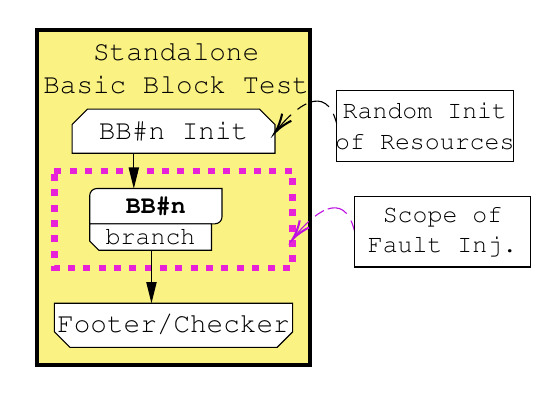
\begin{tikzpicture}[x=0.75pt,y=0.75pt,yscale=-0.85,xscale=0.85]
%uncomment if require: \path (0,385); %set diagram left start at 0, and has height of 385

%Shape: Rectangle [id:dp7916834050251116] 
\draw  [fill={rgb, 255:red, 248; green, 231; blue, 28 }  ,fill opacity=0.54 ][line width=1.5]  (375,140) -- (530,140) -- (530,330) -- (375,330) -- cycle ;
%Snip Same Side Corner Rect [id:dp7832878745055954] 
\draw  [fill={rgb, 255:red, 255; green, 255; blue, 255 }  ,fill opacity=1 ] (395,193.75) -- (403.75,185) -- (501.25,185) -- (510,193.75) -- (510,210) -- (510,210) -- (395,210) -- (395,210) -- cycle ;
%Shape: Rectangle [id:dp19676599731675015] 
\draw  [color={rgb, 255:red, 230; green, 33; blue, 215 }  ,draw opacity=1 ][dash pattern={on 2.53pt off 3.02pt}][line width=2.25]  (385,220) -- (520,220) -- (520,275) -- (385,275) -- cycle ;
%Rounded Diagonal Corner Rect [id:dp03911783521924184] 
\draw  [fill={rgb, 255:red, 255; green, 255; blue, 255 }  ,fill opacity=1 ] (405,234) .. controls (405,231.79) and (406.79,230) .. (409,230) -- (480,230) .. controls (480,230) and (480,230) .. (480,230) -- (480,246) .. controls (480,248.21) and (478.21,250) .. (476,250) -- (405,250) .. controls (405,250) and (405,250) .. (405,250) -- cycle ;
%Snip Single Corner Rect [id:dp49029702843535405] 
\draw  [fill={rgb, 255:red, 255; green, 255; blue, 255 }  ,fill opacity=1 ] (474.01,265) -- (410.25,265) -- (405,259.75) -- (405,250) -- (474.01,250) -- cycle ;
%Straight Lines [id:da003741804416257599] 
\draw    (440,265) -- (440,275) ;
%Straight Lines [id:da6294090718838072] 
\draw    (430,210) -- (430,228) ;
\draw [shift={(430,230)}, rotate = 270] [fill={rgb, 255:red, 0; green, 0; blue, 0 }  ][line width=0.08]  [draw opacity=0] (12,-3) -- (0,0) -- (12,3) -- cycle    ;
%Shape: Rectangle [id:dp024127327494653628] 
\draw   (545,174.5) -- (645,174.5) -- (645,214.5) -- (545,214.5) -- cycle ;
%Curve Lines [id:da39814587147130376] 
\draw  [dash pattern={on 3.75pt off 3pt on 7.5pt off 1.5pt}]  (545,193.25) .. controls (538.89,169.12) and (521.29,184.11) .. (511.08,196.87) ;
\draw [shift={(510,198.25)}, rotate = 307.57] [color={rgb, 255:red, 0; green, 0; blue, 0 }  ][line width=0.75]    (10.93,-3.29) .. controls (6.95,-1.4) and (3.31,-0.3) .. (0,0) .. controls (3.31,0.3) and (6.95,1.4) .. (10.93,3.29)   ;
%Curve Lines [id:da23423265564935447] 
\draw [color={rgb, 255:red, 189; green, 16; blue, 224 }  ,draw opacity=1 ] [dash pattern={on 3.75pt off 3pt on 7.5pt off 1.5pt}]  (555,253.75) .. controls (548.89,229.62) and (531.29,244.61) .. (521.08,257.37) ;
\draw [shift={(520,258.75)}, rotate = 307.57] [color={rgb, 255:red, 189; green, 16; blue, 224 }  ,draw opacity=1 ][line width=0.75]    (10.93,-3.29) .. controls (6.95,-1.4) and (3.31,-0.3) .. (0,0) .. controls (3.31,0.3) and (6.95,1.4) .. (10.93,3.29)   ;
%Shape: Rectangle [id:dp4792679092541773] 
\draw   (555,234.5) -- (655,234.5) -- (655,274.5) -- (555,274.5) -- cycle ;
%Snip Same Side Corner Rect [id:dp19614433052146063] 
\draw  [fill={rgb, 255:red, 255; green, 255; blue, 255 }  ,fill opacity=1 ] (520,311.25) -- (511.25,320) -- (393.75,320) -- (385,311.25) -- (385,295) -- (385,295) -- (520,295) -- (520,295) -- cycle ;
%Straight Lines [id:da35004371293914116] 
\draw    (440,275) -- (440,287.67) -- (440,293) ;
\draw [shift={(440,295)}, rotate = 270] [fill={rgb, 255:red, 0; green, 0; blue, 0 }  ][line width=0.08]  [draw opacity=0] (12,-3) -- (0,0) -- (12,3) -- cycle    ;

% Text Node
\draw (454,162) node   [align=left] {\begin{minipage}[lt]{100.64pt}\setlength\topsep{0pt}
\begin{center}
{\fontfamily{pcr}\selectfont Standalone }\\{\fontfamily{pcr}\selectfont Basic Block Test}
\end{center}

\end{minipage}};
% Text Node
\draw (452.5,197.5) node   [align=left] {{\fontfamily{pcr}\selectfont BB\#n Init}};
% Text Node
\draw (439.5,257.5) node  [font=\small] [align=left] {{\fontfamily{pcr}\selectfont branch}};
% Text Node
\draw (442.5,240) node  [font=\small] [align=left] {{\fontfamily{pcr}\selectfont \textbf{BB\#n}}};
% Text Node
\draw (595,194.5) node  [font=\small] [align=left] {\begin{minipage}[lt]{68.82pt}\setlength\topsep{0pt}
\begin{center}
{\fontfamily{pcr}\selectfont Random Init }\\{\fontfamily{pcr}\selectfont of Resources}
\end{center}

\end{minipage}};
% Text Node
\draw (605,254.5) node  [font=\small] [align=left] {\begin{minipage}[lt]{57.8pt}\setlength\topsep{0pt}
\begin{center}
{\fontfamily{pcr}\selectfont Scope of}\\{\fontfamily{pcr}\selectfont Fault Inj.}
\end{center}

\end{minipage}};
% Text Node
\draw (452.5,307.5) node   [align=left] {{\fontfamily{pcr}\selectfont Footer/Checker}};


\end{tikzpicture}
    \caption{Block Diagram of the Entire SW Product}
    \label{complete_sw}
\end{figure}

Although having the set of basic blocks divided in single file may seem sufficient, there still the need to initialize all the resources that both the processor and the basic block itself need to run properly, as well as a control logic to ensure that the functionalities of the basic block are preserved (or not) throughout the course of the fault injection campaign. As Shown in fig:2 a \textbf{random} initialization is included in the header for the basic block, ensuring the non dependability of the reliability metrics extracted on the input data, together with a footer that checks the functionalities of the block itself. Notice that in in this case, contrary of what is done in the Hardware methodology, there is no physical probing of the circuit on which the program or the testbench is running. In this study only the functional aspect of the Software Product under test is observed.


\begin{figure}[ht]
    \centering

\tikzset{every picture/.style={line width=0.75pt}} %set default line width to 0.75pt        

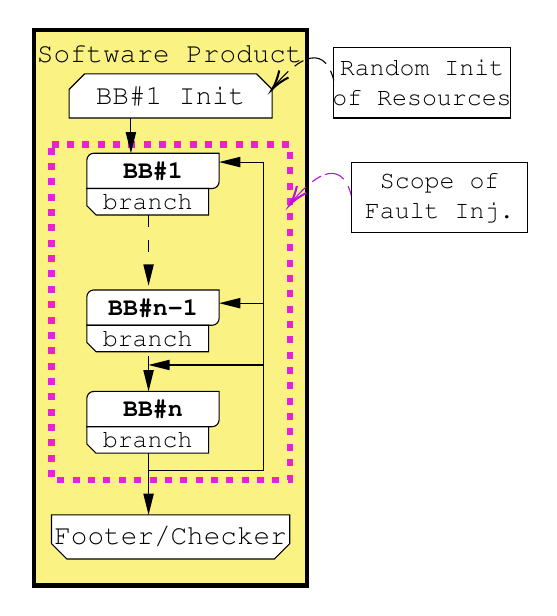
\begin{tikzpicture}[x=0.75pt,y=0.75pt,yscale=-0.85,xscale=0.85]
%uncomment if require: \path (0,385); %set diagram left start at 0, and has height of 385

%Shape: Rectangle [id:dp7802817346854477] 
\draw  [fill={rgb, 255:red, 248; green, 231; blue, 28 }  ,fill opacity=0.54 ][line width=1.5]  (375,25) -- (530,25) -- (530,340) -- (375,340) -- cycle ;
%Snip Same Side Corner Rect [id:dp4511869170411664] 
\draw  [fill={rgb, 255:red, 255; green, 255; blue, 255 }  ,fill opacity=1 ] (395,58.75) -- (403.75,50) -- (501.25,50) -- (510,58.75) -- (510,75) -- (510,75) -- (395,75) -- (395,75) -- cycle ;
%Rounded Diagonal Corner Rect [id:dp4147933552058153] 
\draw  [fill={rgb, 255:red, 255; green, 255; blue, 255 }  ,fill opacity=1 ] (405,99) .. controls (405,96.79) and (406.79,95) .. (409,95) -- (480,95) .. controls (480,95) and (480,95) .. (480,95) -- (480,111) .. controls (480,113.21) and (478.21,115) .. (476,115) -- (405,115) .. controls (405,115) and (405,115) .. (405,115) -- cycle ;
%Straight Lines [id:da5031724996809185] 
\draw  [dash pattern={on 4.5pt off 4.5pt}]  (440,130) -- (440,168) ;
\draw [shift={(440,170)}, rotate = 270] [fill={rgb, 255:red, 0; green, 0; blue, 0 }  ][line width=0.08]  [draw opacity=0] (12,-3) -- (0,0) -- (12,3) -- cycle    ;
%Shape: Rectangle [id:dp3861789631911239] 
\draw  [color={rgb, 255:red, 230; green, 33; blue, 215 }  ,draw opacity=1 ][dash pattern={on 2.53pt off 3.02pt}][line width=2.25]  (385,90) -- (520,90) -- (520,280) -- (385,280) -- cycle ;
%Snip Single Corner Rect [id:dp4150717653667523] 
\draw  [fill={rgb, 255:red, 255; green, 255; blue, 255 }  ,fill opacity=1 ] (474.01,130) -- (410.25,130) -- (405,124.75) -- (405,115) -- (474.01,115) -- cycle ;
%Rounded Diagonal Corner Rect [id:dp6179685400839223] 
\draw  [fill={rgb, 255:red, 255; green, 255; blue, 255 }  ,fill opacity=1 ] (405,176.5) .. controls (405,174.29) and (406.79,172.5) .. (409,172.5) -- (480,172.5) .. controls (480,172.5) and (480,172.5) .. (480,172.5) -- (480,188.5) .. controls (480,190.71) and (478.21,192.5) .. (476,192.5) -- (405,192.5) .. controls (405,192.5) and (405,192.5) .. (405,192.5) -- cycle ;
%Snip Single Corner Rect [id:dp9495482868480547] 
\draw  [fill={rgb, 255:red, 255; green, 255; blue, 255 }  ,fill opacity=1 ] (474.01,207.5) -- (410.25,207.5) -- (405,202.25) -- (405,192.5) -- (474.01,192.5) -- cycle ;
%Rounded Diagonal Corner Rect [id:dp7104472219464535] 
\draw  [fill={rgb, 255:red, 255; green, 255; blue, 255 }  ,fill opacity=1 ] (405,234) .. controls (405,231.79) and (406.79,230) .. (409,230) -- (480,230) .. controls (480,230) and (480,230) .. (480,230) -- (480,246) .. controls (480,248.21) and (478.21,250) .. (476,250) -- (405,250) .. controls (405,250) and (405,250) .. (405,250) -- cycle ;
%Snip Single Corner Rect [id:dp13966897176597148] 
\draw  [fill={rgb, 255:red, 255; green, 255; blue, 255 }  ,fill opacity=1 ] (474.01,265) -- (410.25,265) -- (405,259.75) -- (405,250) -- (474.01,250) -- cycle ;
%Straight Lines [id:da7034569303289814] 
\draw    (440,210) -- (440,228) ;
\draw [shift={(440,230)}, rotate = 270] [fill={rgb, 255:red, 0; green, 0; blue, 0 }  ][line width=0.08]  [draw opacity=0] (12,-3) -- (0,0) -- (12,3) -- cycle    ;
%Straight Lines [id:da744196070297434] 
\draw    (505,100) -- (505,275) ;
%Straight Lines [id:da9733245046694632] 
\draw    (505,100) -- (482,100) ;
\draw [shift={(480,100)}, rotate = 360] [fill={rgb, 255:red, 0; green, 0; blue, 0 }  ][line width=0.08]  [draw opacity=0] (12,-3) -- (0,0) -- (12,3) -- cycle    ;
%Straight Lines [id:da8637960575028926] 
\draw    (505,180) -- (482,180) ;
\draw [shift={(480,180)}, rotate = 360] [fill={rgb, 255:red, 0; green, 0; blue, 0 }  ][line width=0.08]  [draw opacity=0] (12,-3) -- (0,0) -- (12,3) -- cycle    ;
%Straight Lines [id:da16371070865734882] 
\draw    (505,215) -- (442,215) ;
\draw [shift={(440,215)}, rotate = 360] [fill={rgb, 255:red, 0; green, 0; blue, 0 }  ][line width=0.08]  [draw opacity=0] (12,-3) -- (0,0) -- (12,3) -- cycle    ;
%Straight Lines [id:da9354977054242168] 
\draw    (440,265) -- (440,275) ;
%Straight Lines [id:da46391232910603153] 
\draw    (440,275) -- (505,275) ;
%Straight Lines [id:da2767877128184162] 
\draw    (430,75) -- (430,93) ;
\draw [shift={(430,95)}, rotate = 270] [fill={rgb, 255:red, 0; green, 0; blue, 0 }  ][line width=0.08]  [draw opacity=0] (12,-3) -- (0,0) -- (12,3) -- cycle    ;
%Shape: Rectangle [id:dp6690781431266354] 
\draw   (545,35) -- (645,35) -- (645,75) -- (545,75) -- cycle ;
%Curve Lines [id:da6302549466986412] 
\draw  [dash pattern={on 3.75pt off 3pt on 7.5pt off 1.5pt}]  (545,53.75) .. controls (538.89,29.62) and (521.29,44.61) .. (511.08,57.37) ;
\draw [shift={(510,58.75)}, rotate = 307.57] [color={rgb, 255:red, 0; green, 0; blue, 0 }  ][line width=0.75]    (10.93,-3.29) .. controls (6.95,-1.4) and (3.31,-0.3) .. (0,0) .. controls (3.31,0.3) and (6.95,1.4) .. (10.93,3.29)   ;
%Curve Lines [id:da19217143664609126] 
\draw [color={rgb, 255:red, 189; green, 16; blue, 224 }  ,draw opacity=1 ] [dash pattern={on 3.75pt off 3pt on 7.5pt off 1.5pt}]  (555,119.25) .. controls (548.89,95.12) and (531.29,110.11) .. (521.08,122.87) ;
\draw [shift={(520,124.25)}, rotate = 307.57] [color={rgb, 255:red, 189; green, 16; blue, 224 }  ,draw opacity=1 ][line width=0.75]    (10.93,-3.29) .. controls (6.95,-1.4) and (3.31,-0.3) .. (0,0) .. controls (3.31,0.3) and (6.95,1.4) .. (10.93,3.29)   ;
%Shape: Rectangle [id:dp9047170935038439] 
\draw   (555,100) -- (655,100) -- (655,140) -- (555,140) -- cycle ;
%Snip Same Side Corner Rect [id:dp9299469266370497] 
\draw  [fill={rgb, 255:red, 255; green, 255; blue, 255 }  ,fill opacity=1 ] (520,316.25) -- (511.25,325) -- (393.75,325) -- (385,316.25) -- (385,300) -- (385,300) -- (520,300) -- (520,300) -- cycle ;
%Straight Lines [id:da35158879367292817] 
\draw    (440,275) -- (440,287.67) -- (440,298) ;
\draw [shift={(440,300)}, rotate = 270] [fill={rgb, 255:red, 0; green, 0; blue, 0 }  ][line width=0.08]  [draw opacity=0] (12,-3) -- (0,0) -- (12,3) -- cycle    ;

% Text Node
\draw (452,39) node   [align=left] {{\fontfamily{pcr}\selectfont Software Product}};
% Text Node
\draw (452.5,62.5) node   [align=left] {{\fontfamily{pcr}\selectfont BB\#1 Init}};
% Text Node
\draw (439.5,122.5) node  [font=\small] [align=left] {{\fontfamily{pcr}\selectfont branch}};
% Text Node
\draw (442.5,105) node  [font=\small] [align=left] {{\fontfamily{pcr}\selectfont \textbf{BB\#1}}};
% Text Node
\draw (439.5,200) node  [font=\small] [align=left] {{\fontfamily{pcr}\selectfont branch}};
% Text Node
\draw (442.5,182.5) node  [font=\small] [align=left] {{\fontfamily{pcr}\selectfont \textbf{BB\#n-1}}};
% Text Node
\draw (439.5,257.5) node  [font=\small] [align=left] {{\fontfamily{pcr}\selectfont branch}};
% Text Node
\draw (442.5,240) node  [font=\small] [align=left] {{\fontfamily{pcr}\selectfont \textbf{BB\#n}}};
% Text Node
\draw (595,55) node  [font=\small] [align=left] {\begin{minipage}[lt]{68.82pt}\setlength\topsep{0pt}
\begin{center}
{\fontfamily{pcr}\selectfont Random Init }\\{\fontfamily{pcr}\selectfont of Resources}
\end{center}

\end{minipage}};
% Text Node
\draw (605,120) node  [font=\small] [align=left] {\begin{minipage}[lt]{57.8pt}\setlength\topsep{0pt}
\begin{center}
{\fontfamily{pcr}\selectfont Scope of}\\{\fontfamily{pcr}\selectfont Fault Inj.}
\end{center}

\end{minipage}};
% Text Node
\draw (452.5,312.5) node   [align=left] {{\fontfamily{pcr}\selectfont Footer/Checker}};


\end{tikzpicture}
    \caption{Block Diagram of the Entire SW Product}
    \label{complete_sw}
\end{figure}


\subsection{Fault Injection on Randomly Initialized Resources}

Fault injection is the mean by which the misbehavior and faulty execution is provoked on purpose on digital systems. In the past, especially on hardware, fault injection was aimed to functionally verify the designs under test. Those DUT were analysed, their functions (data dependent) extracted and inputs were selected in order to exercise those functions. Later on the fault injection had the role of determining whether those functions were preserved in cases of fault or how eventually they were modified. Today this is still the state of the art for software verification.

With time a second approach on hardware was presented, testing moved from functional to structural, where the integrity of the device is evaluated, regardless of the function (and therefore of data), verifying solely the implemented boolean function.

The methodology introduced in this paper presents the novelty of applying this structural approach to software. To abstract the basic block as much as possible from its link to data, \textbf{every resource utilized has been randomized} before each fault injection. The probability of failure and propagation probabilities are therefore extracted \textbf{independently} of their data input.

Probes (i.e., observation points) are defined during the setup of the fault injection campaign. It is the role of the Footer/Checker (out of the scope of the fault injection) to redirect the output of the block function into a reserved portion of the memory to be probed. Probes are set on those reserved memory location on all blocks, not probing the correctness of the data with respect to the golden run, but solely if the basic function included in that portion of code has been affected by the fault injection. 

\subsection{Re-Composition of the basic blocks}
Once the fault injection campaigns are over, it is time to re-compose the information that have been extracted on the single blocks into a complete description of the original Software Product. To perform the re-composition there is the need run the software once and record the trace, this will allow us to know exactly the sequence in which the basic blocks have been executed during the nominal run.  

We distinguish two main branches of the re-composition, the ones containing fault that \textit{do not modity the program flow} and those that lead to a \textit{modified program flow} 
\subsubsection{Not modified Program Flow}
First we nee to define the probability of being executing a precise basic block in time during the execution of the program. Assuming a deterministic duration per executed instruction, without nested or hidden operation, we can define the probability of executing $BB_n$ as 
\begin{equation}
    P_{in-bb_n} = \frac{instructions-in-BB_n}{total-instruction-in-exe}
\end{equation}
Next step is to define the probability of a fault happening in $BB_n$ being able to become an error in the same block. This has been deduced from fault injection and must be differentiated per every register in which we inject faults and it represented as:
\begin{equation}
    P^{A_m}_{gBB_n}
\end{equation}
Last probability to define is the probability of a block to receive a wrong input and propagate it to its output. Defined as:
\begin{equation}
    P^{A_m}_{pBB_n} 
\end{equation}
which is related to the "time of life" of the variables, defined as the number of basic block between the last time a variable has been read and the first time it gets overwritten.



Once these probabilities ha been defined we can describe the worst possible case, in which a fault is injected in $BB_n$ and gets propagated throughout the whole program. 
\begin{align}
    \begin{split}
        & P_{in-bb_n} * P^{A_m}_{gBB_n} * \left[ P^{A_m}_{pBB_{n+1}} \dots P^{A_m}_{pBB_{f}}\right] +
   \\ &+  P_{in-bb_{n+1}} * P^{A_m}_{gBB_{n+1}} * \left[ P^{A_m}_{pBB_{n+2}} \dots P^{A_m}_{pBB_{f}}\right]\dots   
    \end{split}
\end{align}    



which summarizes, per every register $A_m$ as:

\begin{equation}
    	\sum_{n=0}^N  P_{in-bb_n} * P^{A_m}_{gBB_n} *\left[ \prod_{i=n}^N  \left[ P^{A_m}_{pBB_{i+1}} \right]\right]
\end{equation}



\begin{equation}
    P_{tot} = [P_{in-bb-x} * P_{p-bbx}] + [P_{p-bbx+1} * P_{p-bbx+1}]  \dots
\end{equation}
\subsubsection{Modified Program Flow}
Regarding the possibility of having a fault injected on a register while the program is executing a precise Basic Block that requires a branching operation at the end, we cannot consider them while recomposing the metrics as in the previous subsection.

These blocks contribute instead to the composition of a particular subset of runs (diverse behaviour of the program) which include all those runs in which the program simulation has reached the end in a time that differs from the nominal one. In particular, it can be shortened due to a premature jump to the conclusive part of the program as well as delayed due to an incorrect loop that sends the machine into a non-necessary series of states from which it will eventually recover. In the case in which the machine would not be able to recover, we categorize those runs as Timeouts (when longer than 150\% of nominal time).\textit{ It worth to point out that, due to the nature of the injections, which focus on the Register file, with one SEU per run, these cases are reduced to the minimum, if not nonexistent.}
Give these assumptions, taking into account this second section of Basic Blocks, it is possible to assume that most, if not all of these runs will generate a failure in the functionalities of the program itself. therefore the recomposition, that was missing a good half of what was neded, now finds the missing cases in all those blocks that led to a modification in the flow.

In particular, considering the possibility that this blocks have not to propagate (to mask) a fault occurring in the course of their routine, the event of flow corruption has probability $1 - P_{masking}$, then the probability of these fault becoming a funcional error is $100\%$ and it does not propagate.
In this case the recomposition technique is slightly different than the previous section, as the case of a missed branch or jump leads directly to an error. So defined the multiplicity of the same critical block in the nominal sequence $m$, the probability of having a functinoal failure is described by:
\begin{equation}
    P_{err} + P_{msk} * P_{err} + (P_{msk})^{2} * P_{err} \cdots + (P_{msk})^m * P_{err}
\end{equation}

Taking into accoun the approximation due to the algorithm intrinsic ability to recover from a flow error.

%
%~~~~~~~~~~~~~~~~~~~~~~~~~~~~~~~~~~~~~~~~~~~~~~~~~~~~~~~~~~~~~~~~~~~~~~~~~~~~
%                       TESTCASE
%~~~~~~~~~~~~~~~~~~~~~~~~~~~~~~~~~~~~~~~~~~~~~~~~~~~~~~~~~~~~~~~~~~~~~~~~~~~~
%

\section{Test Case and Application}
\label{sec:testcase}
\subsection{The Software}
The Software of choice for the Proof of Concept of this methodology is the Bubble Sort Algoritm, in its Assembler for RISC-V Version. Bubble sort is an $O(n^2)$ sorting algorithm. A simple sorting algorithm that performs a one-way comparison of two adjacent records from the head to tail of the disordered part in each sort trip. Of course, the direction can also be the contrary, one-way comparison from the tail to head of the disordered part. This will form gradually an ordered table at the head of the disordered table, and the basic idea of the algorithm has no difference with the foregoing \cite{5635119}.


\subsection{The Division in Basic Block}
The processing of dividing the Software under test into basic block has been carried out automatically and returned 8 different blocks, together with the list of resources that each and every basic blocks utilizes during its own functions.
After a Nominal run without faults of the entire software, it was possible to trace the transition between the different basic blocks throughout the whole execution. These information, summarized in the scheme below, will be the key to predict the behaviour of the program starting from the behaviour of the basic blocks themselves.

\begin{figure}[h]
    \centering




\tikzset{every picture/.style={line width=0.75pt}} %set default line width to 0.75pt        

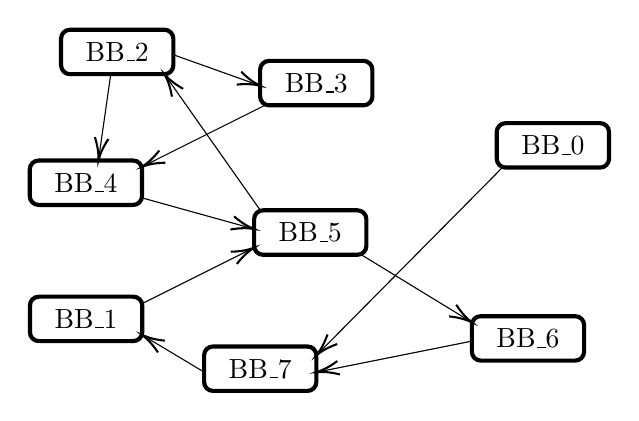
\begin{tikzpicture}[x=0.75pt,y=0.75pt,yscale=-1,xscale=1]
%uncomment if require: \path (0,385); %set diagram left start at 0, and has height of 385

%Rounded Rect [id:dp8950193773121069] 
\draw  [line width=1.5]  (251.91,67.28) .. controls (251.91,64.92) and (253.82,63) .. (256.19,63) -- (301.72,63) .. controls (304.08,63) and (306,64.92) .. (306,67.28) -- (306,80.12) .. controls (306,82.49) and (304.08,84.4) .. (301.72,84.4) -- (256.19,84.4) .. controls (253.82,84.4) and (251.91,82.49) .. (251.91,80.12) -- cycle ;
%Rounded Rect [id:dp9984058842626251] 
\draw  [line width=1.5]  (27,150.88) .. controls (27,148.51) and (28.92,146.6) .. (31.28,146.6) -- (76.81,146.6) .. controls (79.18,146.6) and (81.09,148.51) .. (81.09,150.88) -- (81.09,163.72) .. controls (81.09,166.08) and (79.18,168) .. (76.81,168) -- (31.28,168) .. controls (28.92,168) and (27,166.08) .. (27,163.72) -- cycle ;
%Rounded Rect [id:dp9856513256588806] 
\draw  [line width=1.5]  (137.91,37.28) .. controls (137.91,34.92) and (139.82,33) .. (142.19,33) -- (187.72,33) .. controls (190.08,33) and (192,34.92) .. (192,37.28) -- (192,50.12) .. controls (192,52.49) and (190.08,54.4) .. (187.72,54.4) -- (142.19,54.4) .. controls (139.82,54.4) and (137.91,52.49) .. (137.91,50.12) -- cycle ;
%Rounded Rect [id:dp901157696578387] 
\draw  [line width=1.5]  (26.91,85.28) .. controls (26.91,82.92) and (28.82,81) .. (31.19,81) -- (76.72,81) .. controls (79.08,81) and (81,82.92) .. (81,85.28) -- (81,98.12) .. controls (81,100.49) and (79.08,102.4) .. (76.72,102.4) -- (31.19,102.4) .. controls (28.82,102.4) and (26.91,100.49) .. (26.91,98.12) -- cycle ;
%Rounded Rect [id:dp24680170852961525] 
\draw  [line width=1.5]  (135,109.28) .. controls (135,106.92) and (136.92,105) .. (139.28,105) -- (184.81,105) .. controls (187.18,105) and (189.09,106.92) .. (189.09,109.28) -- (189.09,122.12) .. controls (189.09,124.49) and (187.18,126.4) .. (184.81,126.4) -- (139.28,126.4) .. controls (136.92,126.4) and (135,124.49) .. (135,122.12) -- cycle ;
%Rounded Rect [id:dp33862831913115987] 
\draw  [line width=1.5]  (239.91,160.28) .. controls (239.91,157.92) and (241.82,156) .. (244.19,156) -- (289.72,156) .. controls (292.08,156) and (294,157.92) .. (294,160.28) -- (294,173.12) .. controls (294,175.49) and (292.08,177.4) .. (289.72,177.4) -- (244.19,177.4) .. controls (241.82,177.4) and (239.91,175.49) .. (239.91,173.12) -- cycle ;
%Rounded Rect [id:dp1757835836146553] 
\draw  [line width=1.5]  (110.91,174.88) .. controls (110.91,172.51) and (112.82,170.6) .. (115.19,170.6) -- (160.72,170.6) .. controls (163.08,170.6) and (165,172.51) .. (165,174.88) -- (165,187.72) .. controls (165,190.08) and (163.08,192) .. (160.72,192) -- (115.19,192) .. controls (112.82,192) and (110.91,190.08) .. (110.91,187.72) -- cycle ;
%Rounded Rect [id:dp18264707725482388] 
\draw  [line width=1.5]  (42,22.28) .. controls (42,19.92) and (43.92,18) .. (46.28,18) -- (91.81,18) .. controls (94.18,18) and (96.09,19.92) .. (96.09,22.28) -- (96.09,35.12) .. controls (96.09,37.49) and (94.18,39.4) .. (91.81,39.4) -- (46.28,39.4) .. controls (43.92,39.4) and (42,37.49) .. (42,35.12) -- cycle ;
%Straight Lines [id:da3712867751572613] 
\draw    (138,105) -- (92.96,41.04) ;
\draw [shift={(91.81,39.4)}, rotate = 54.85] [color={rgb, 255:red, 0; green, 0; blue, 0 }  ][line width=0.75]    (10.93,-3.29) .. controls (6.95,-1.4) and (3.31,-0.3) .. (0,0) .. controls (3.31,0.3) and (6.95,1.4) .. (10.93,3.29)   ;
%Straight Lines [id:da3337276101977069] 
\draw    (66,39) -- (60.28,79.02) ;
\draw [shift={(60,81)}, rotate = 278.13] [color={rgb, 255:red, 0; green, 0; blue, 0 }  ][line width=0.75]    (10.93,-3.29) .. controls (6.95,-1.4) and (3.31,-0.3) .. (0,0) .. controls (3.31,0.3) and (6.95,1.4) .. (10.93,3.29)   ;
%Straight Lines [id:da3195921749278837] 
\draw    (96,30) -- (136.12,44.33) ;
\draw [shift={(138,45)}, rotate = 199.65] [color={rgb, 255:red, 0; green, 0; blue, 0 }  ][line width=0.75]    (10.93,-3.29) .. controls (6.95,-1.4) and (3.31,-0.3) .. (0,0) .. controls (3.31,0.3) and (6.95,1.4) .. (10.93,3.29)   ;
%Straight Lines [id:da3950293151484261] 
\draw    (141,54) -- (82.79,83.11) ;
\draw [shift={(81,84)}, rotate = 333.43] [color={rgb, 255:red, 0; green, 0; blue, 0 }  ][line width=0.75]    (10.93,-3.29) .. controls (6.95,-1.4) and (3.31,-0.3) .. (0,0) .. controls (3.31,0.3) and (6.95,1.4) .. (10.93,3.29)   ;
%Straight Lines [id:da7859903078227688] 
\draw    (81,99) -- (133.07,113.46) ;
\draw [shift={(135,114)}, rotate = 195.52] [color={rgb, 255:red, 0; green, 0; blue, 0 }  ][line width=0.75]    (10.93,-3.29) .. controls (6.95,-1.4) and (3.31,-0.3) .. (0,0) .. controls (3.31,0.3) and (6.95,1.4) .. (10.93,3.29)   ;
%Straight Lines [id:da22105063899115163] 
\draw    (81,150) -- (133.21,123.89) ;
\draw [shift={(135,123)}, rotate = 153.43] [color={rgb, 255:red, 0; green, 0; blue, 0 }  ][line width=0.75]    (10.93,-3.29) .. controls (6.95,-1.4) and (3.31,-0.3) .. (0,0) .. controls (3.31,0.3) and (6.95,1.4) .. (10.93,3.29)   ;
%Straight Lines [id:da18941500229563069] 
\draw    (111,183) -- (82.71,166.03) ;
\draw [shift={(81,165)}, rotate = 30.96] [color={rgb, 255:red, 0; green, 0; blue, 0 }  ][line width=0.75]    (10.93,-3.29) .. controls (6.95,-1.4) and (3.31,-0.3) .. (0,0) .. controls (3.31,0.3) and (6.95,1.4) .. (10.93,3.29)   ;
%Straight Lines [id:da8800586209378064] 
\draw    (186,126) -- (238.29,157.96) ;
\draw [shift={(240,159)}, rotate = 211.43] [color={rgb, 255:red, 0; green, 0; blue, 0 }  ][line width=0.75]    (10.93,-3.29) .. controls (6.95,-1.4) and (3.31,-0.3) .. (0,0) .. controls (3.31,0.3) and (6.95,1.4) .. (10.93,3.29)   ;
%Straight Lines [id:da8051529089918902] 
\draw    (240,168) -- (166.96,182.61) ;
\draw [shift={(165,183)}, rotate = 348.69] [color={rgb, 255:red, 0; green, 0; blue, 0 }  ][line width=0.75]    (10.93,-3.29) .. controls (6.95,-1.4) and (3.31,-0.3) .. (0,0) .. controls (3.31,0.3) and (6.95,1.4) .. (10.93,3.29)   ;
%Straight Lines [id:da13132970852441106] 
\draw    (255,84) -- (166.41,173.46) ;
\draw [shift={(165,174.88)}, rotate = 314.72] [color={rgb, 255:red, 0; green, 0; blue, 0 }  ][line width=0.75]    (10.93,-3.29) .. controls (6.95,-1.4) and (3.31,-0.3) .. (0,0) .. controls (3.31,0.3) and (6.95,1.4) .. (10.93,3.29)   ;

% Text Node
\draw (278.95,73.7) node   [align=left] {BB\_0};
% Text Node
\draw (54.05,157.3) node   [align=left] {BB\_1};
% Text Node
\draw (164.95,43.7) node   [align=left] {BB\_3};
% Text Node
\draw (53.95,91.7) node   [align=left] {BB\_4};
% Text Node
\draw (162.05,115.7) node   [align=left] {BB\_5};
% Text Node
\draw (266.95,166.7) node   [align=left] {BB\_6};
% Text Node
\draw (137.95,181.3) node   [align=left] {BB\_7};
% Text Node
\draw (69.05,28.7) node   [align=left] {BB\_2};


\end{tikzpicture}

    \caption{Block Diagram of the Entire SW Product}
    \label{complete_sw}
\end{figure}




\subsection{The Platform}
The choice of the platform on which the program has been run and tested fell on the SCR1SOC. SCR1 is an open-source and free to use RISC-V compatible MCU-class core, designed and maintained by Syntacore. It is industry-grade and silicon-proven (including full-wafer production), works out of the box in all major EDA flows and Verilator, and comes with extensive collateral and documentation \cite{}. This choice had mostly been driven by the larger and larger usage of these kind of RISCV based cores in the academic community. Any test based on these platforms is and added value to their development. 

\subsection{The Fault Injection Campaign}
The next step in the methodology is fault injection. It is performed using Cadence fault injection tool {\it FSV} \cite{ICM}. Once fault injection sites are automatically identified from the RTL description, fault injection is performed and 20 faults are injected per identified site using a custom pre-generated fault dictionary, including a random injection time. An in-house tool build on top of the {\it GSL} \cite{GSL} has been developed for this purpose. Such number is statistically significant enough \cite{5090716} without compromising fault injection campaign running time. Faults are injected on the integrity of the register file, mimic as well the possibility of faults propagated to the memory and back. Also, fault probes are set on non excerciced memory location to record which injected faults will cause a functional failure of the basic block. For each fault injection run, a logfile is generated which reports the outcome of the run, later a custom made parsing tool will recollect the data from this logfile and present the results to the re-composition tool.

 


%
%~~~~~~~~~~~~~~~~~~~~~~~~~~~~~~~~~~~~~~~~~~~~~~~~~~~~~~~~~~~~~~~~~~~~~~~~~~~~
%                       RESULT AND DISCUSSION
%~~~~~~~~~~~~~~~~~~~~~~~~~~~~~~~~~~~~~~~~~~~~~~~~~~~~~~~~~~~~~~~~~~~~~~~~~~~~

\section{Scalability}
Evaluating the efficacy and scalability of a methodology can be a complex and demanding undertaking, particularly when the algorithm under examination possesses a high time complexity. It is imperative to establish the impartiality and reliability of the results obtained through the evaluation process. To accomplish this, the methodology was subjected to multiple trials, each utilizing a distinct and randomly selected data set with varying lengths, resulting in a diversity of execution times.

\begin{table}[H]
\centering
\begin{tabular}{|c|c|c|}
\hline
\textbf{Number of Elements} & \textbf{Execution Time (us)} & \textbf{Simulation Time} \\
\hline
\hline
10 & 180.2050 & 00:00:10 \\
\hline
25 & 775.5250 & 00:00:13 \\
\hline
50 & 3130.4850 & 00:00:39 \\
\hline
100 & 12135.846868 & 00:02:24 \\
\hline
250 & 77431.1650 & 00:13:50 \\
\hline
500 & 304928.3250 & 00:55:38 \\
\hline
\end{tabular}
\caption{Time data}
\label{table:time_data}
\end{table}


The utilization of various data sets, each of differing size, eliminates the possibility of biases and guarantees a thorough evaluation of the methodology. The range of execution times provides an assessment of the scalability of the methodology, and any limitations can be identified. Moreover, the consistent outcomes across all trials serve as robust proof for the validity of the results.

A graphical representation of the progression and evolution of the data through the multiple iterations is presented, which underscores the consistency of the results, regardless of differences in data size and execution time. This consistency further reinforces the impartiality and reliability of the results and boosts confidence in the validity of the methodology under examination.

It is worth mentioning that the scalability of the methodology is also influenced by the high complexity of the algorithm being evaluated, in this case, with a time complexity of $O(n^2)$. Despite this, the impartiality and reliability of the results were maintained through the repeated trials, each utilizing a unique and randomly selected data set.

In summary, the methodology evaluation process was executed in a systematic and thorough manner, ensuring the impartiality and reliability of the results obtained. The use of multiple data sets, each with varying lengths, and the consistent outcomes across all trials provide strong proof for the validity of the methodology under examination. The graphical representation further supports the impartiality and reliability of the results and instills confidence in the scalability and efficacy of the methodology.


\section{Results and Future Work}
The results of the recomposition are based on Table:1, which summarizes the result of the fault injection campaign that has been carried out on the single basic blocks. Each entry of the table enumerates the number of functional error on caused by each register in the register file, keeping in mind that every bit in the register has been affected by 20 faults randomized in time, for a total of 640 faults per register. Once these table has been given to the recomposition tool, Table:2 is returned, including the benchmark fault injection campaign on the entire Software Product for validation of results together with the expected number of faults, calculated following the methodology described. Last, Table:3 Reports the number of Errors that have been caused by an error in the flow of the program, which can be extracted by an equivalent of table number 1 for flow errors caused by each register failing in each basic block and recomposed as in its dedicated section.

\newgeometry{left=1cm, right =1cm, bottom=1cm, top=1cm} 
\begin{table}[H]
    \centering
    \caption{Result of Fault Injection on basic blocks}
    \begin{tabular}{|l|l|l|l|l|l|l|l|l|l|l|l|l|l|l|l|l|l|l|l|}
    \hline
        ~ & x0 & x1 & x2 & x3 & x4 & x5 & x6 & x7 & x8 & x9 & x10 & x11 & x12 & x13 & x14 & x15 & x16 & ~ & x31 \\ \hline
        bb\_0 & 0 & 0 & 139 & 0 & 0 & 0 & 0 & 0 & 379 & 0 & 0 & 0 & 0 & 0 & 0 & 162 & 0 & ... & 0 \\ \hline
        bb\_1 & 0 & 0 & 0 & 0 & 0 & 0 & 0 & 0 & 500 & 0 & 0 & 0 & 0 & 0 & 0 & 0 & 0 & ... & 0 \\ \hline
        bb\_2 & 0 & 0 & 0 & 0 & 0 & 0 & 0 & 0 & 269 & 0 & 0 & 0 & 0 & 28 & 14 & 38 & 0 & ... & 0 \\ \hline
        bb\_3 & 0 & 0 & 0 & 0 & 0 & 0 & 0 & 0 & 500 & 0 & 0 & 0 & 0 & 16 & 131 & 244 & 0 & ... & 0 \\ \hline
        bb\_4 & 0 & 0 & 0 & 0 & 0 & 0 & 0 & 0 & 495 & 0 & 0 & 0 & 0 & 0 & 0 & 62 & 0 & ... & 0 \\ \hline
        bb\_5 & 0 & 0 & 0 & 0 & 0 & 0 & 0 & 0 & 380 & 0 & 0 & 0 & 0 & 0 & 0 & 0 & 0 & ... & 0 \\ \hline
        bb\_6 & 0 & 0 & 0 & 0 & 0 & 0 & 0 & 0 & 494 & 0 & 0 & 0 & 0 & 0 & 0 & 41 & 0 & ... & 0 \\ \hline
        bb\_7 & 0 & 0 & 0 & 0 & 0 & 0 & 0 & 0 & 466 & 0 & 0 & 0 & 0 & 0 & 0 & 0 & 0 & ... & 0 \\ \hline
    \end{tabular}
\end{table}

\begin{table}[H]
    \centering
    \caption{Comparison of Fault Injection data vs Recomposed data on Entire Software}
    \begin{tabular}{|l|l|l|l|l|l|l|l|l|l|l|l|l|l|l|l|l|l|l|l|}
    \hline
        ~ & x0 & x1 & x2 & x3 & x4 & x5 & x6 & x7 & x8 & x9 & x10 & x11 & x12 & x13 & x14 & x15 & x16 & ~ & x31 \\ \hline
        FI & 0 & 0 & 4 & 0 & 0 & 0 & 0 & 0 & 221 & 0 & 0 & 0 & 0 & 15 & 41 & 90 & 0 & ... & 0 \\ \hline
        Reco & 0 & 0 & 5 & 0 & 0 & 0 & 0 & 0 & 228 & 0 & 0 & 0 & 0 & 13 & 44 & 98 & 0 & ... & 0 \\ \hline
    \end{tabular}
\end{table}

\begin{table}[H]
    \centering
    \caption{Control Flow Driven Errors}
    \begin{tabular}{|l|l|l|l|l|l|l|l|l|l|l|l|l|l|l|l|l|l|l|l|}
    \hline
        ~ & x0 & x1 & x2 & x3 & x4 & x5 & x6 & x7 & x8 & x9 & x10 & x11 & x12 & x13 & x14 & x15 & x16 & ~ & x31 \\ \hline
        FI & 0 & 0 & 0 & 0 & 0 & 0 & 0 & 0 & 198 & 0 & 0 & 0 & 0 & 4 & 77 & 90 & 0 & ... & 0 \\ \hline
        RECO & 0 & 0 & 0 & 0 & 0 & 0 & 0 & 0 & 205 & 0 & 0 & 0 & 0 & 6 & 70 & 93 & 0 & ... & 0 \\
        \hline
    \end{tabular}
\end{table}
\restoregeometry



The last part of the methodology will be the focus of the work to come, as includes the implicit ability of the different algorithms to recover from flow errors, which understanding can lead to much more refined results.
\label{sec:discussion}




\end{document}
